\chapter{Background}\label{chap:background}
To predict the next element in a running case, we bring together the domains of Process Science, Predictive Modeling and Deep Learning. This background chapter gives comprehensive insight into those parts of said domains which will be used and referenced in this thesis. The chapter approaches them in a top-down fashion, starting with the high-level perspective from Process Science and how Process Mining is distinguished from Predictive Process Monitoring in \autoref{sec:process-science}. The section ends with information on how the used logs usually come into existence and which requirements these logs need to fulfill to be used in a prediction scenario.
With the data origin explained, \autoref{sec:predictive-modeling} introduces the KDD process, along which predictive model development usually takes place.
\autoref{sec:artificial-neural-networks} gives an in-depth look at neural networks and the components relevant to this thesis, especially stressing the importance of long short-term memory cells.
Finally, \autoref{sec:background:feature-engineering} highlights the peculiarities encountered when dealing with sequential data and introduces popular approaches to deal with them.

\section{Process Science And Process Monitoring}\label{sec:process-science}
Process Science, as loosely defined by van der Aalst~\cite{Aalst2016}, refers to the \textit{broader discipline that combines knowledge from information technology and knowledge from management sciences to improve and run operational processes}. This results in improvement approaches that tend to be driven by process models.

These models can be defined in a variety of modeling languages~\cite{panagacos2012ultimate}. Most languages, for example the Business Process Modeling Notation (BPMN)~\cite{bpmn2.0}, model the process flow in steps, commonly referred to as \textit{activities}, and shown in \autoref{fig:activity-introduction}. Less rigid are the models found in Adaptive Case Management (ACM), where rigidity is traded for flexibility during process execution. The latter sees more application in the domain of knowledge work, but both have an important detail in common: events.

\begin{figure}
    \centering
    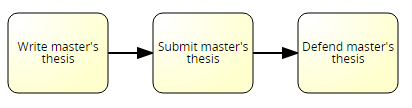
\includegraphics[width=.75\textwidth]{gfx/activity-introduction.png}
    \caption{The yellow boxes and their description are used in BPMN to describe an activity. The arrows denote the control flow in between.}
    \label{fig:activity-introduction}
\end{figure}

With the help of workflow management systems (WFMS), it is possible to embed and enforce structured processes in an organization. These systems log events related to each activity, e.g. once it starts or ends. Said event logs give rise to the disciplines of Process Mining and Predictive Process Monitoring, as their analyses rest on the information contained therein\cite{Aalst2016}. \autoref{sec:process-mining} and \autoref{sec:predictive-process-monitoring} contrast these very similar domains and how they can be distinguished. Finally, \autoref{sec:log-structure} formally defines the properties a log needs to fulfill to be considered useful for analysis. In the following, the execution history of a single case is also referred to as \textit{trace}.

\begin{figure}
    \centering
    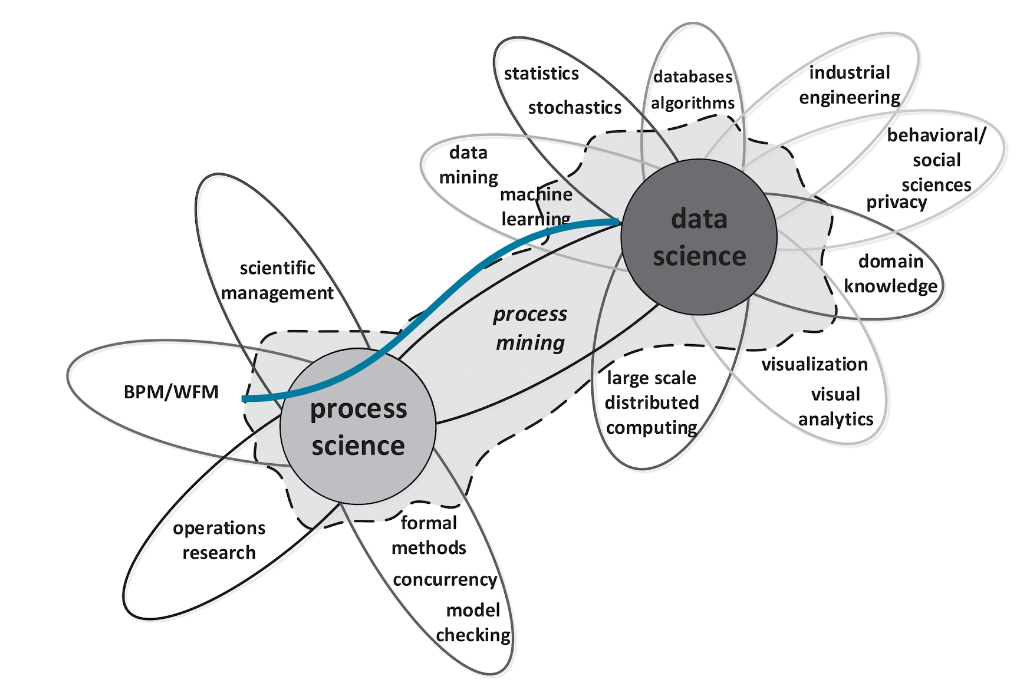
\includegraphics[width=.8\textwidth]{gfx/process-data-science.png}
    \caption{Process Mining can be understood as the bridge between Process Science and Data Science \cite[p.18]{Aalst2016}. The blue line symbolizes the subdomains that Predictive Process Monitoring brings together.}
    \label{fig:process-data-science}
\end{figure}

\subsection{Process Mining}\label{sec:process-mining}
Process Mining covers the three steps of process model discovery, conformance checking and process model enhancement \cite{Aalst2016} -  all enabled by the aforementioned process execution logs. These individual steps are made possible by techniques from the area of Data Science, making it possible to understand Process Mining as a link between Data Science and Process Science as in \autoref{fig:process-data-science}.

A major problem in this domain is posed by \textit{spaghetti} and \textit{lasagna} process models\cite{Aalst2016}. Such overly complex and unreadable models are mined from process logs that contain highly variable execution traces. These traces often come from ACM executions.

Because Process Mining revolves around process models, and the data-driven discovery and optimization based on historical data, a possibility to act on case developments in real-time without model-imposed restrictions is desirable.

\subsection{Predictive Process Monitoring}
\label{sec:predictive-process-monitoring}
A young domain aiming at the use of online data to make statements about the progression of a running case is that of \textit{Predictive Process Monitoring}~\cite{francescomarino2015, schoenig2018}, thus fulfilling the aforementioned need. The application of Predictive Analytics on incomplete traces connects two sub-domains of Process Science and Data Science, setting it apart from the model-focused Process Mining. This is also illustrated in \autoref{fig:process-data-science}.

Instead of revolving around models, this discipline is concerned with predicting characteristics of running cases. This allows answering questions such as:

\begin{enumerate}
    \item Can the service level agreement still be met?
    \item How long is this case still going to take?
    \item What is going to be the next step in the case?
\end{enumerate}

The answers to these questions can give case workers the opportunity to intervene if a case takes an unwanted course or might fail to meet requirements or key performance indicators. Furthermore, this approach only requires sufficient amounts of historical case executions, but no model. While a model can certainly be a useful addition, it is not needed. Especially the last point stands in strong connection to the rising popularity of ACM, since a process model previously dictated the possible choices for the next activity.

\subsection{Process execution log requirements}\label{sec:log-structure}
\begin{figure}
    \centering
    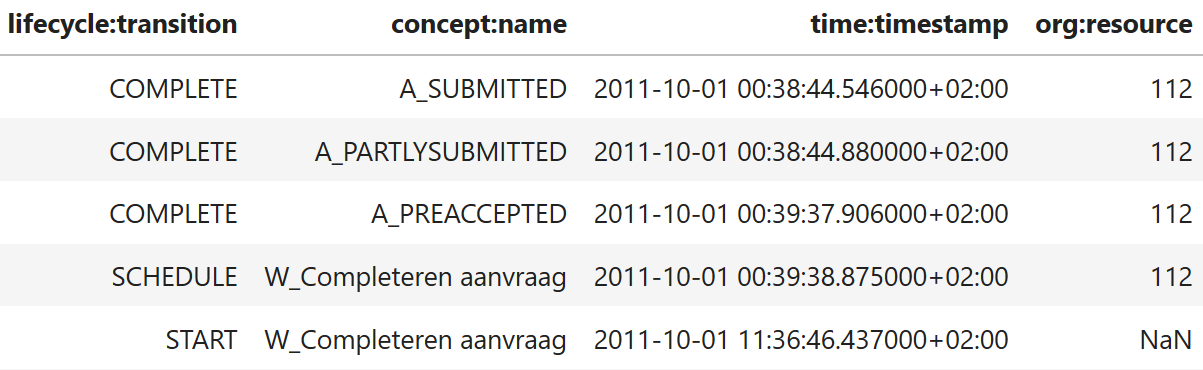
\includegraphics[width=\textwidth]{gfx/process-log.png}
    \caption{The first entries of an exemplary event log from a case from the BPIC 2011 dataset~\cite{BPIC2011}. Each event is associated with data; column \texttt{concept:name} corresponds to the activity title.}
    \label{fig:process-log}
\end{figure}

An exemplary log suited for analysis is depicted in \autoref{fig:process-log}, which was extracted from an XES-formatted file.
XES is an abbreviation for the \textit{eXtensible Event Stream} standard, commonly used for process event logs~\cite{gunther2013xes}. As the execution of a process activity can take a certain amount of time, process \textit{events} are used to distinguish between e.g. the start or end of an activity. These events are contained inside these logs, together forming a trace.

A log can be made up of any number of traces $t \in T$, where each trace $t$ represents an ordered number of events $e \in E$:

$$ t = \langle e_1, e_2, e_3 \dots \rangle $$

In turn, each event $e$ has certain attributes associated with it. It is assumed that in a log for a specific process, the type, number and name of these attributes does not change. An example for a type of such a data attribute is the activity name or the timestamp at which this event occurred. Thus, an event represents a set of attributes, in which only one attribute $d_i$ of a specific type $C_i$ occurs:

$$ e = \{ d_1, d_2, d_3, ..., d_i\ |\ d_i \in C_i \}$$

In this formulation, each $C_i$ maps onto a column like in \autoref{fig:process-log}, and each $e$ onto a row. With this structure, a log lends itself for application in the context of Predictive Modeling, as the next section will show.

\section{Predictive Modeling}
\label{sec:predictive-modeling}
Predictive Modeling is a domain that deals with creating models from learned statistical properties of data to predict outcomes. The models used to arrive at these outcomes are referred to as predictive models, and are unrelated to process models. This section introduces a common process for predictive model generation in \autoref{sec:predictive-model-development} and frames a problem in \autoref{sec:background:sequence-prediction} that is fundamental to the thesis: that of next-element predictions in a sequence.

\subsection{Predictive model development}
\label{sec:predictive-model-development}
\begin{figure}
	\centering
	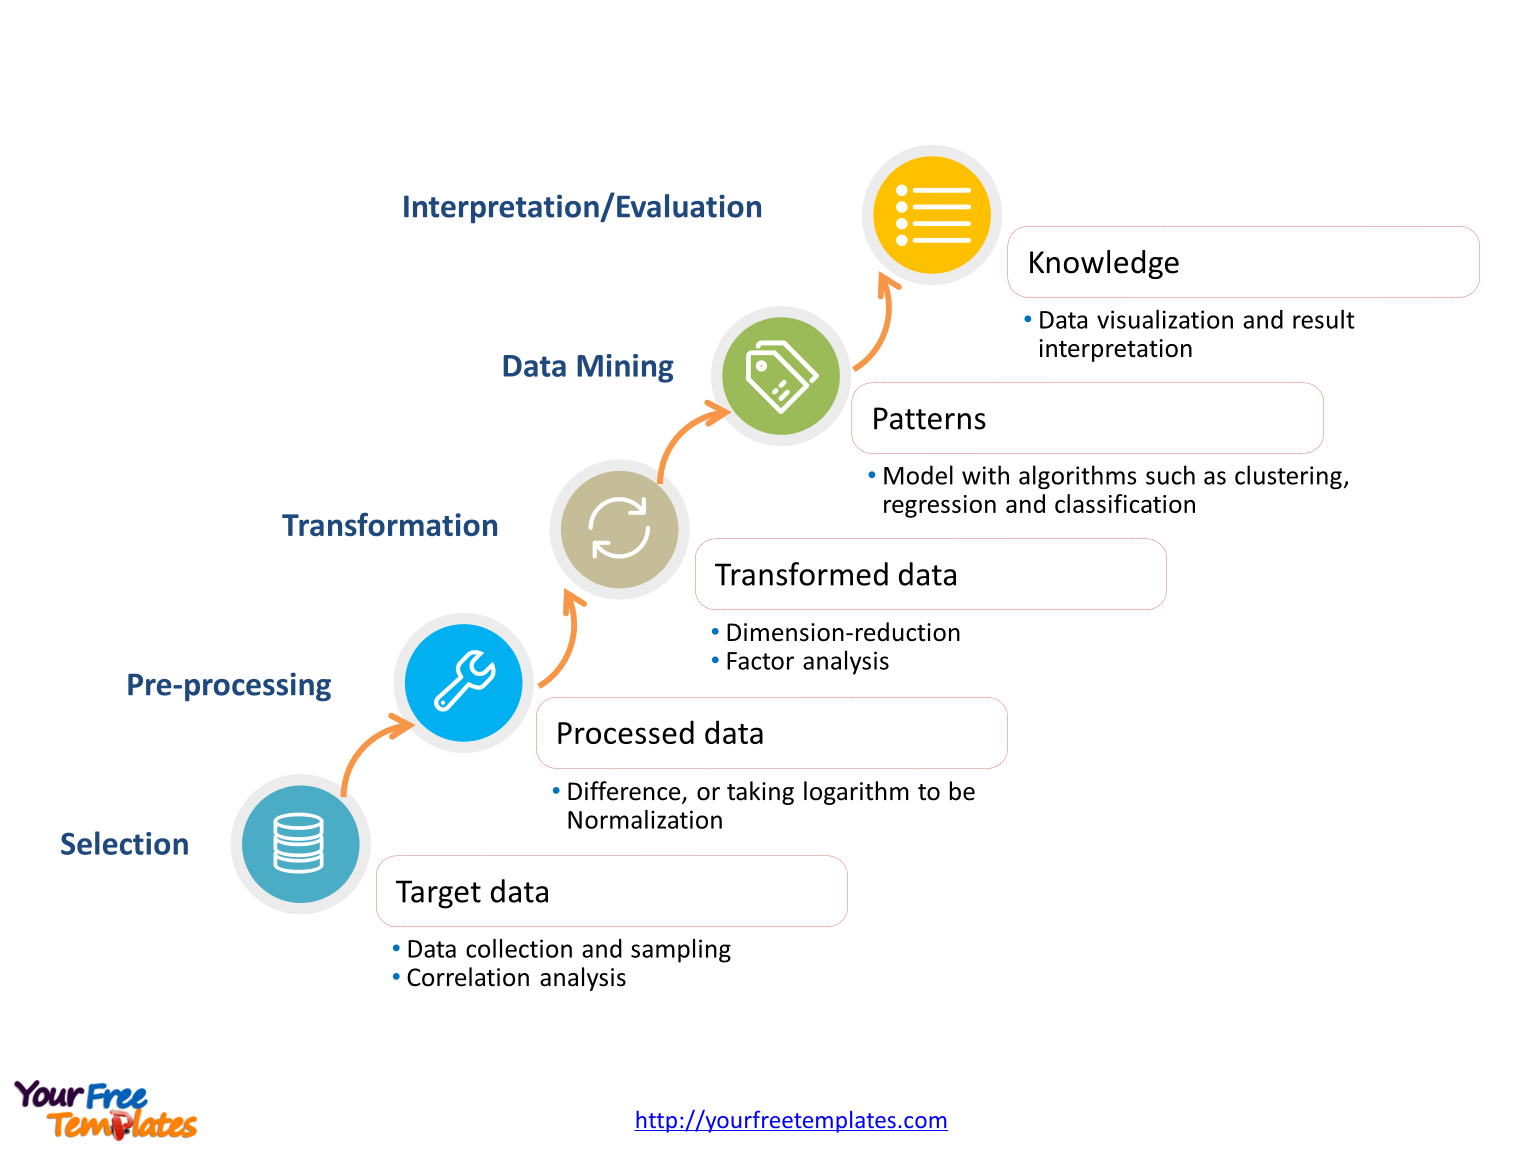
\includegraphics[width=\textwidth]{gfx/kdd_process.png}
	\caption{The process for \textit{Knowledge Discovery in Databases} as per Fayyad et al. \cite{fayyad1996data}.}
	\label{fig:kdd_process}
\end{figure}

In 1996 Fayyad et al. published what came to be known as the Knowledge Discovery In Databases (KDD) process \cite{fayyad1996data}. Published 20 years ago and aimed at data mining, it is also applicable to predictive model building. It is illustrated in \autoref{fig:kdd_process}, and shall be explained step by step in the following with technical details relevant for this thesis. The process is highly iterative and jumps between every step are possible.

\subsubsection*{Selection}
Predictive models work on \textit{line items} comprised of a number of \textit{features}, which are variables that are considered useful for the prediction of the \textit{target variable}. The target variable may either be a continuous or discrete value. In the latter case, the output is referred to as classification. Activities are discrete, and this thesis deals with classification.
In the exemplary log in \autoref{fig:process-log}, each row is a line item and each column corresponds to a single feature. Features are sometimes also referred to as predictor variables.

During the selection step features are chosen as predictors based on differed criteria such as their predictive power or inter-feature correlations.

\subsubsection*{Pre-processing}
Some features may be sparse or contain data of low-quality. With methods from the area of data cleansing, these issues are resolved and appropriate values imputed for missing features. When using event logs, it is important to only use those parts that belong to a specific process. Furthermore, concept drift needs to be taken into account.

\subsubsection*{Transformation}
\label{sec:predictive-model-development:transformation}
During transformation, some features might be aggregated, normalized or differently encoded to assist the model in picking up relations between variables. Common tasks are one-hot or dictionary encoding of discrete values such as strings, e.g. activity names. Variable concatenations or complex aggregations might also be added as separate \textit{engineered} features \cite{schoenig2018}.

\subsubsection*{Data Mining}
The goal of predicting the next activity is a classification task. For this type of task, a wide array of applicable predictive models is available, such as decision trees, random forests, support vector machines (SVM) or artificial neural networks (ANN).

The data prepared in the previous steps is used to \textit{train} the model. During this training phase, the model uses accuracy metrics to assess the quality of its predictions, learn the statistical properties of the data and adjust its internals accordingly. Certain input parameters of the model are adjusted during this phase as well, an activity referred to as \textit{hyper-parameter tuning}. Training the model can be a very time-consuming task, unless appropriate hardware is used. Certain pieces of hardware speed up model learning (i.e. Google's Tensor Processing Units) or a simple Graphics Processing Unit (GPU).

\subsubsection*{Evaluation}
Typically, not all of the available data is used for training. This is to make sure that the model generalizes well, i.e. predicts as good on data it is has not seen before as on the training data. If a model is not generalizing, it is said to be \textit{overfitting}. Overfitting happens when the model is strongly biased towards the training data too well and thus shows poor generalization performance. A simple and effective method to avoid biases is to divide the available data into three parts: 50\% of it to train the model, 25\% of it to calculate and improve the model during training and the remaining 25\% to finally test the model performance after training~\cite{kuhn2013applied, trevor2009elements}.

\subsection{Sequence prediction}\label{sec:background:sequence-prediction}
A sequence is made up of individual steps. This section presents a formal definition of sequences, which will later be used to connect process traces with the process prediction problem at hand. Let $I = \{i_1, i_2, \cdots, i_n\}$ be the set of all items. An \textit{itemset} $s$ is a subset of $I$. A \textit{sequence} $seq$ is an ordered list of itemsets, such that it can be noted as follows:

$$seq = \langle s_1s_2\cdots s_l \rangle\ |\ \forall\ 0 \leq j \leq l: s_j \subseteq I$$

Then, $S$ defines the infinite set of all possible sequences. It is infinite because sequences can be arbitrarily long, with each itemset containing an arbitrary number of items. For  subsequences, the notation $seq_{i,k}$ denotes the containment of the elements from index $i$ through $k$ from the original sequence: $seq_{1,2} = \langle s_1s_2 \rangle$.\\

Assuming that a sequence finishes eventually, consider the database of finished sequences $DS$. Under the assumption of the Markovian hypothesis that "the probability of each event depends only on the state attained in the previous event"~\cite{gagniuc2017markov}, a predictive model can be trained on this database to predict the next sequence $nseq$ or itemset $s_k$ of an incomplete sequence $seq_{inc}$:

\begin{equation}
\begin{split}
    predict(seq_{inc}) &= \widehat{nseq}\\
    predict(seq_{inc}) &= \hat{s_k}\ |\ 0 \leq k \leq l
\end{split}
\label{eq:prediction-from-sequence}
\end{equation}

Sequence predictions are a common problem in the domains of machine translation and text generation. For example, the translation of the sentence \textit{"I am writing my master's thesis"} into the german sentence \textit{"Ich schreibe meine Masterarbeit"} can easily be mapped onto the notation previously described. With $I$ being the alphabet and each itemset representing a single word, the input and target sequences could be noted as:

\begin{equation*}
\begin{split}
seq_{EN} &= \langle<I> <am> <writing> <my> <thesis>\rangle\\
seq_{GER} &= \langle<Ich> <schreibe> <meine> <Masterarbeit>\rangle
\end{split}
\end{equation*}

Referring to \autoref{eq:prediction-from-sequence}, $seq_{EN}$ can be understood as the argument to $predict$, and $seq_{GER}$ as $\widehat{nseq}$. This is a simple example of a \textit{sequence-to-sequence} prediction.

Next to this kind of prediction, there are also \textit{sequence-to-word} predictions, which can be used to generate text and even write simple novels~\cite{web:text-generation-machinelearningmastery, web:text-generation-freecodecamp}. The transfer of this general formulation onto the translation problem is easy to imagine, since the prediction target of a sequence need not be a word of an incomplete sentence - it could also be the name of an activity of an incomplete trace. The connection of the sequence definition to process logs is presented in \autoref{chap:taking-inspiration}.

\subsection{The curse of dimensionality}
The curse of dimensionality is a term used across various domains such as combinatorics, sampling optimization and machine learning to describe phenomena that arise when working with data data in high-dimensional spaces.

Common to all domains is the fact that an increase in dimensionality increases the volume of the solution space so fast that the data quickly becomes sparse. This eventually causes problems for algorithms which require statistic significance, which again would require an increase in the amount of data to produce.
Because of this, increasing the number of features for training a predictive model, only helps to a certain extent when the number of training samples is constant, as \autoref{fig:dimensionality-vs-performance} illustrates.

\begin{figure}
    \centering
    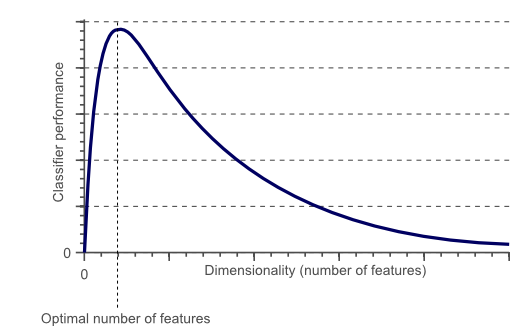
\includegraphics[width=.75\textwidth]{gfx/dimensionality_vs_performance.png}
    \caption{Increasing the feature space does not improve model performance indefinitely}
    \label{fig:dimensionality-vs-performance}
\end{figure}

\section{Artificial Neural Networks}\label{sec:artificial-neural-networks}
An artificial neural network (ANN) mimics the inner workings of a human brain in that it is made up of connected nodes referred to as neurons. These neurons are interconnected and act on the incoming signals from each connection. This section first gives background on the general structure of a classic neural network in \autoref{sec:feedforward-networks} and then highlights two enhancements for sequence learning in \autoref{sec:recurrent-networks} and \autoref{sec:lstm}.

\subsection{Feedforward neural networks}
\label{sec:feedforward-networks}
\begin{figure}[ht!]
    \centering
    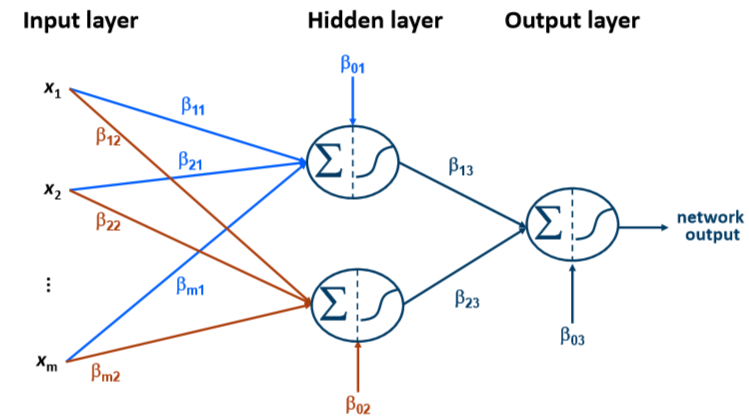
\includegraphics[width=.85\textwidth]{gfx/feedforward-neural-network.png}
    \caption{A simple feed-forward ANN with a single hidden layer. The network takes the inputs $x_1$ to $x_m$ and passes them through edges that are weighted with weights $\beta_{ij}$. Illustration taken from \cite{lessmannBADS}}
    \label{fig:feedforward-ann}
\end{figure}

The nodes are organized in layers, with each neuron connecting to every neuron in the adjacent layers, resulting in fully connected layers. The layers between the input and output layers are referred to as \textit{hidden layers} and  can be greater in number. The signal at an edge between neurons is a number, and the output of each artificial neuron is computed by a function of the sum of its inputs. This function is called \textit{activation function}, as it decides whether the neuron emits a signal or not. \autoref{fig:feedforward-ann} showcases the edges, their weights, and the activation function in a very simple ANN architecture. As $x_1$ to $x_m$ are fed in at once, the input to a neural network is often referred to as input vector.

Edges are weighted with the weights being adjusted as the learning proceeds. During training, data is passed from layer to layer in synchronized steps. This is done in \textit{batches} - after each batch the weights are adjusted. The passing of all training data through the network is called an \textit{epoch}.

The weight adjustment happens according to the result of the \textit{loss function}, which calculates how far the network's predictions missed the training data. The goal of the training algorithm is thus to minimize the loss, which can lead to overfitting if the loss is optimized for too many epochs.

Feed-forward ANNs are moving their internal signals in a single direction: toward the output layer. This behaviour causes the network not to have any capacity for persisting what it has previously processed. Put simply, it is not able to \textit{remember}.

As the next chapter will show, recurrent neural networks (RNN) have been created with this capacity in mind, making them suited for working with sequential data. Long short-term memory enhances the capacity to remember even further.

\subsection{Recurrent neural networks}\label{sec:recurrent-networks}
As the name suggests, recurrent neural networks (RNN) implement a feedback loop. This loop makes information from the output of a neuron available to that same neuron for the next step. Taking the time dimension into account, RNNs are often displayed in an unrolled fashion as in \autoref{fig:rnn-unrolled}. This form of illustration also reveals that recurrent neural networks are intimately related to sequences and lists.

\begin{figure}
    \centering
    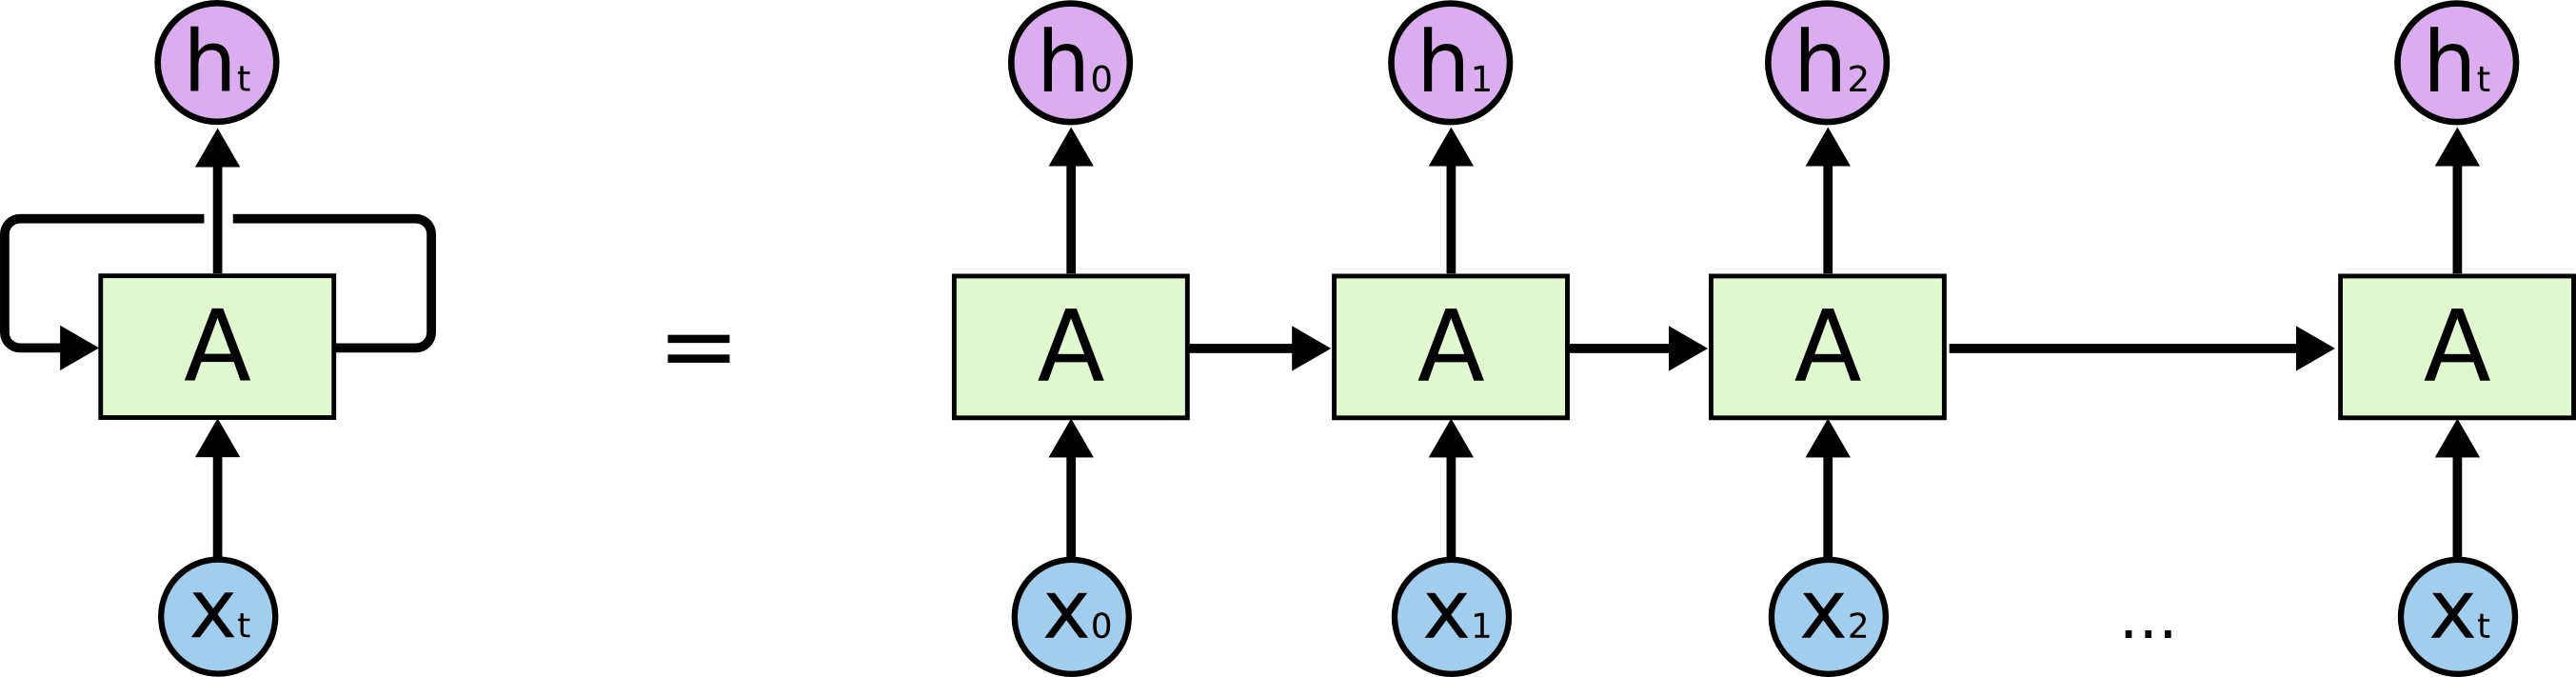
\includegraphics[width=.9\textwidth]{gfx/rnn-unrolled.png}
    \caption{A neuron receives an input $x_t$ and outputs a value $h_t$. The loop allows information to be passed from one step $t$ of the network to the next step $t+1$. This Illustration is taken from \cite{web:colah}}
    \label{fig:rnn-unrolled}
\end{figure}

While the loop indeed allows recognizing short-term dependencies, the network as a whole will still underperform with long-term dependencies when the gaps between related inputs become too great. The root cause is that RNNs lack a memory to bridge those gaps. This problem has been thoroughly explored by Hochreiter et al.~\cite{hochreiter1991untersuchungen} who also proposed the long short-term memory fix presented in the following section.

\subsection{Long short-term memory}\label{sec:lstm}
In recent years, RNNs were applied with great success to a variety of problems: speech recognition, language modeling or translation. This success can be attributed in part to the enhancement of RNNs with long short-term memory (LSTM) cells.

Hochreiter \& Schmidhuber published this enhancement in 1997 \cite{hochreiter1997} which now sees wide application. Essentially, the repeating module of a RNN was equipped with a state, i.e. the capacity to remember. The cell state $C$ is managed through chaining together different operators, one of them also representing a capacity to forget. \autoref{fig:lstm} showcases an unrolled LSTM layer with the cell architecture exposed. Variants of the original LSTM cell architecture exist, with most modifications made on the construction of the state $C$ - all exhibiting very similar performance \cite{greff2017lstm}.

\begin{figure}[ht!]
    \centering
    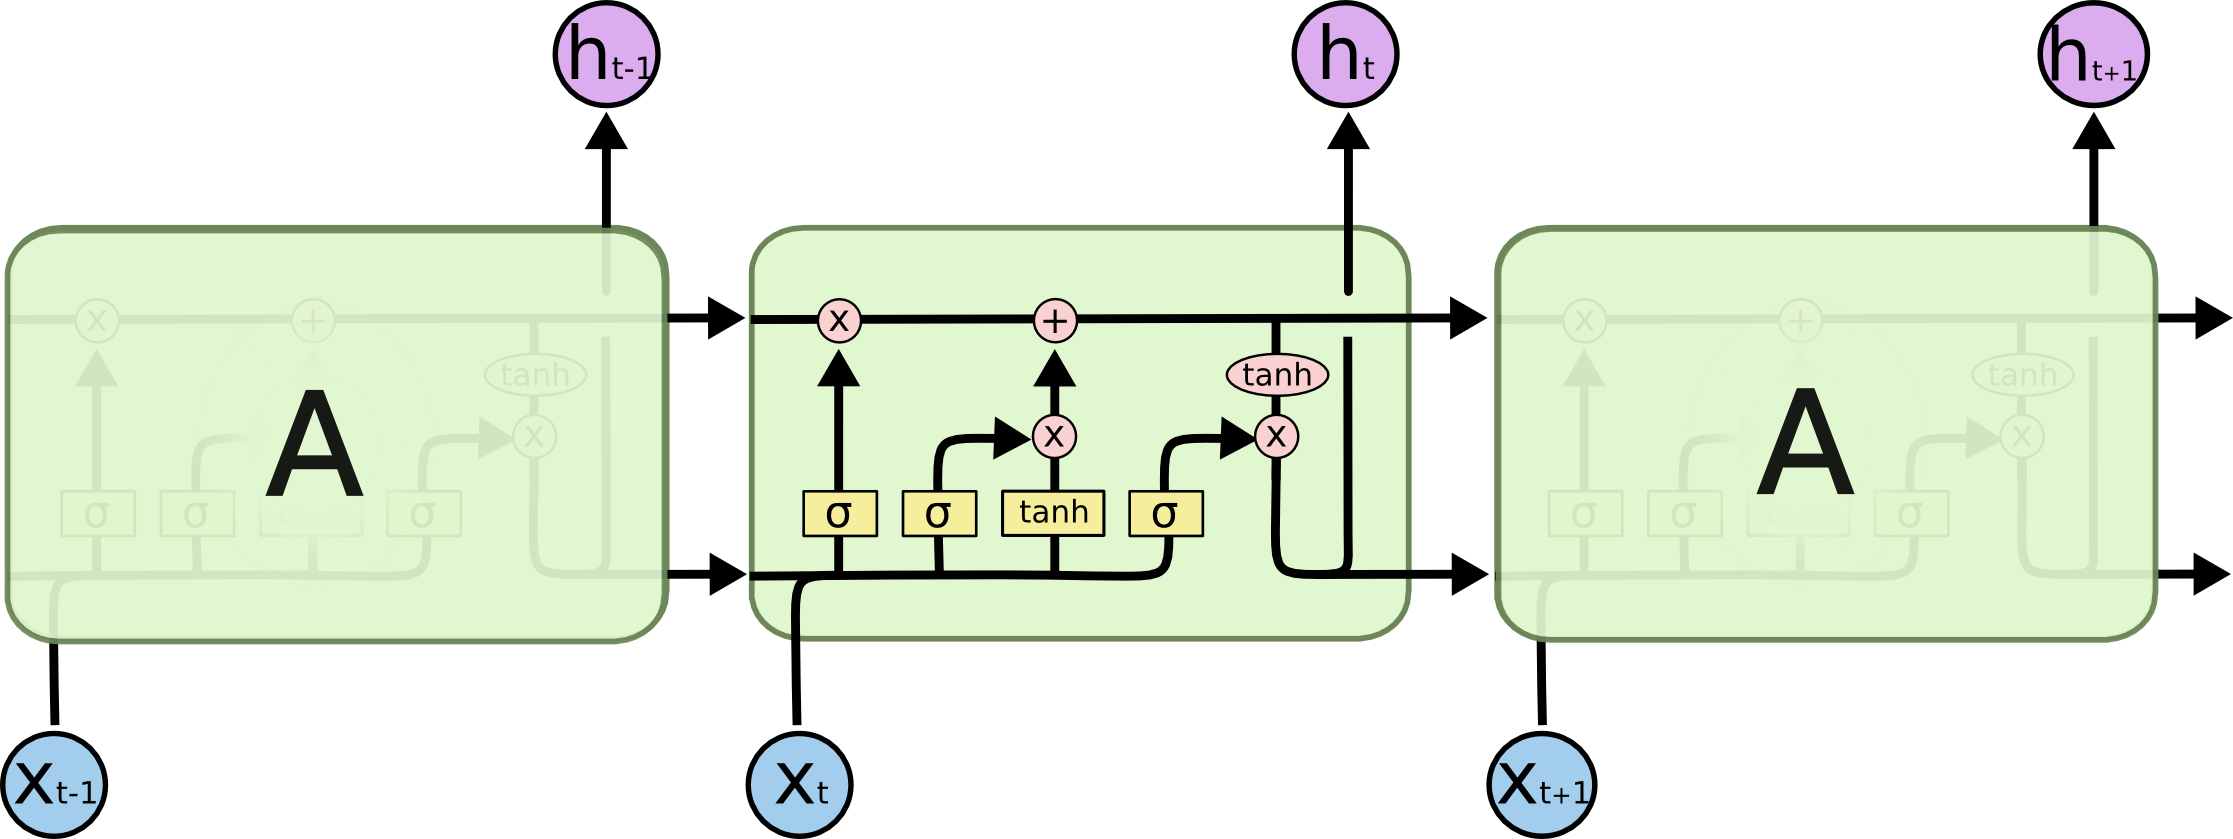
\includegraphics[width=.8\textwidth]{gfx/lstm-chain.png}
    \caption{An exemplary unrolled LSTM repeating module with the upper horizontal line representing the cell state $C$. This Illustration is taken from \cite{web:colah}}
    \label{fig:lstm}
\end{figure}

\section{Data preparation and feature engineering}
\label{sec:background:feature-engineering}
Data preparation and feature engineering are the tasks in predictive model development that demand the most effort and have the greatest impact on prediction performance. To assist predictive models during training, most features need to be reformatted. This section shall highlight the relevant methods used for categorical variables in \autoref{sec:categorical-feature-engineering}. \autoref{sec:sequential-feature-engineering} points out methods with which to make sequential inputs of various length conform with the fixed-width input requirement of predictive models. In the case of ANNs this requirement can easily be explained by the fixed number of units on the input layer. The methods are demonstrated at the example of the following two sequences:
\begin{equation*}
    \begin{split}
        seq1 &= \langle<Arthur>,\ <is>,\ <the>,\ <king>\rangle\\
        seq2 &= \langle<Maria>,\ <wants>,\ <to>,\ <be>,\ <the>,\ <queen>\rangle
    \end{split}
\end{equation*}

\subsection{Feature engineering for categorical features}
\label{sec:categorical-feature-engineering}
While ordinal features are most often normalized, categorical features can be encoded in a variety of ways. Categorical features are e.g. strings like \textit{red} and \textit{black}, which have no numerical format and may or may not be relative to each other. Where one-hot and dictionary encodings are traditional approaches for these features, word embeddings represent a relatively new and promising approach.

\subsubsection*{One-hot encoding}
One-hot encoding is often used for features which have a small to medium-sized number of unique values. Using it, each line item of a feature is expanded to an $n$ column representation, where $n$ represents the number all possible values, also referred to as the alphabet. The columns hold a boolean flag, of which only one is true in any given row, hence the name. This type of encoding is also sometimes referred to as "dummy encoding"~\cite{web:pandas-get-dummies}. Thus, the first word of $seq1$ would be encoded as in \autoref{tab:one-hot}. As the alphabet becomes larger, so does $n$, and so does its sparsity - again leading toward the curse of dimensionality.

\begin{table}[ht]
    \centering
    \begin{tabular}{c|c|c|c|c|c|c|c|c}
        Maria & Arthur & is & wants & to & king & be & the & queen\\
        \hline
        0 & 1 & 0 & 0 & 0 & 0 & 0 & 0 & 0\\
    \end{tabular}
    \caption{One-hot encoding of "Arthur" using the alphabet of $seq1$ and $seq2$.}
    \label{tab:one-hot}
\end{table}

\subsubsection*{Dictionary encoding}
Widely used in compression, for example in in-memory database systems~\cite{plattner2012memory}, dictionary encoding is also used to encode categorical values. Since predictive models only process numerical values, dictionary encoding is used to create a look-up table and map every value of a feature to a numeric code, like in \autoref{tab:dictionary-encoding}.

In contrast to one-hot encoding, this dictionary encoding does not result in wide and sparse inputs, making it suitable for features with a large number of distinct features. However, it has one important ramification: It imposes an order on features which previously might not have had one. In our example, the condition $Maria > Arthur$ holds true after encoding. The dictionary-encoded sequences would look like this:
\begin{equation*}
    \begin{split}
        seq1 &= \langle1\ 2\ 7\ 5\rangle\\
        seq2 &= \langle0\ 3\ 4\ 6\ 7\ 8\rangle
    \end{split}
\end{equation*}

\begin{figure}
    \centering
    \begin{tabular}{c|ccccccccc}
        Word & Maria & Arthur & is & wants & to & king & be & the & queen\\
        \hline
        Code & 0 & 1 & 2 & 3 & 4 & 5 & 6 & 7 & 8
    \end{tabular}
    \caption{The dictionary built from the itemsets of $seq1$ and $seq2$.}
    \label{tab:dictionary-encoding}
\end{figure}

\subsubsection*{Word embedding}
Because dictionary encodings impose an order and one-hot encodings lead to sparsity, word embeddings are perceived as a viable alternative for encoding categorical variables.

A word embedding is the output of a neural network with a single hidden layer that has been trained on a large text corpus and thus detected how words relate to each other \cite{web:word-embedding}. The network puts out highly dimensional vectors for each word which represent any word property that the model has learned. This allows for interesting examples with vector arithmetic, such as the well-known one shown below. In this famous example the network was able to detect gender properties and social semantics of a word.

$$
    \vec{v}_{king} - \vec{v}_{man} + \vec{v}_{women} = \vec{v}_{queen}
$$

A word embedding thus allows clustering of words by certain properties.
Made popular by Google, the most extensively trained word embedding that is publicly available is word2vec~\cite{web:ahogrammer, goldberg2014word2vec}.

\subsection{Feature engineering for sequences}
\label{sec:sequential-feature-engineering}
Predictive models take inputs of fixed size. As shown, sequences can be of arbitrary length, and thus the curse of dimensionality is especially prominent in context with this problem. To bring variable length inputs into a usable format for predictive models, several methods of formatting have been invented. As some of their names names suggest, these come from the domain of Natural Language Processing (NLP), but can easily be transferred to the problem at hand.

\subsubsection*{Sliding Window}
The sliding window format is very common in the areas of NLP and Time Series Forecasting. The sequences are divided into chunks of width $c$. This results in several input tuples for every sequence, and brings the desired tabular format for feeding into the model - illustrated in \autoref{tab:sliding-window}.

\begin{table}[ht]
    \centering
    \begin{tabular}{cc}
        Word 1 & Word 2\\
        \hline
        Arthur & is\\
        is & the\\
        the & king\\
        Maria & wants\\
        wants & to\\
        to & be\\
        be & the\\
        the & queen
    \end{tabular}
    \caption{Windows created from $seq1$ and $seq2$ with $c=2$}
    \label{tab:sliding-window}
\end{table}

\subsubsection*{Bag-Of-Words}
The bag-of-words (BOW) encoding produces $l$ input tuples, the length of the encoded sequence. Similarly to one-hot encoding, all possibly occurring values need to be known. One arrives at the encoding by counting the occurrences of each item or itemset in $seq$ for each subsequence $seq_{1,k}$. As \autoref{tab:bow-encoding} evidences, this type of encoding leads to sparsity, too.

\begin{table}[]
    \centering
    \begin{tabular}{c|ccccccccc}
        Sequence & Maria & Arthur & is & wants & to & king & be & the & queen\\
        \hline
        $seq1_{1,1}$ & 0 & 1 & 0 & 0 & 0 & 0 & 0 & 0 & 0\\
        $seq1_{1,2}$ & 0 & 1 & 1 & 0 & 0 & 0 & 0 & 0 & 0\\
        $seq1_{1,3}$ & 0 & 1 & 1 & 0 & 0 & 0 & 0 & 1 & 0\\
        $seq1_{1,4}$ & 0 & 1 & 1 & 0 & 0 & 1 & 0 & 1 & 0\\
        \hline
        $seq2_{1,1}$ & 1 & 0 & 0 & 0 & 0 & 0 & 0 & 0 & 0\\
        $seq2_{1,2}$ & 1 & 0 & 0 & 1 & 0 & 0 & 0 & 0 & 0\\
        $seq2_{1,3}$ & 1 & 0 & 0 & 1 & 1 & 0 & 0 & 0 & 0\\
        $seq2_{1,4}$ & 1 & 0 & 0 & 1 & 1 & 0 & 1 & 0 & 0\\
        $seq2_{1,5}$ & 1 & 0 & 0 & 1 & 1 & 0 & 1 & 1 & 0\\
        $seq2_{1,5}$ & 1 & 0 & 0 & 1 & 1 & 0 & 1 & 1 & 1\\
    \end{tabular}
    \caption{Bag-of-words encoding for $seq1$ and $seq2$.}
    \label{tab:bow-encoding}
\end{table}
\subsubsection*{$n$-grams}
The $n$-gram approach is very popular in computational linguistics, biology and data compression and is effectively an $(n-1)$-order Markov model, with the most popular choices for $n$ being $1,2$ and $3$. These models would be called \textit{unigram}, \textit{bigram} and \textit{trigram} models.

Similar to BOW, an $n$-gram model counts occurences. Different from BOW however, it tracks the occurence of subsequences of length $n$. Suppose a set $LS$ holds all possible values of a single feature. From $LS$, a feature set $FS$ is constructed with every item being a permutation of length $n$. A feature in this set would be referred to as \textit{gram}, and can also be understood as a possible subsequence.

$$
FS = S(LS, n)
$$

While $n$-grams can be be powerful features to use, their high dimensionality causes high computational loads and sparse data. With the small featureset of 9 words in the given example, a line item using tri-grams would already be $\frac{|FS|!}{(|FS|-n)!}=504$ elements wide and is thus an illustration is omitted here.

\subsubsection*{Subsequence mining}
One of the main weaknesses of $n$-grams is the restriction to a single $n$ and that "one may need to examine a combinatorially explosive
number of possible subsequence patterns" \cite{pei2001prefixspan}. For this reason, approaches have been developed that combine the benefit of $n$-grams with more flexibility by avoiding the limitation to $n$. An algorithms sifts through input sequences and detects sequential patterns of any length. These sequences are then encoded instead of the $n$-grams, resulting in line items similar to the ones in \autoref{tab:bow-encoding}, with the respective boolean entry denoting the occurence of a specific subsequence in the sequence. Examples for these algorithms are GSP \cite{srikant1996gsp}, FreeSpan \cite{han2000freespan} and PrefixSpan \cite{pei2001prefixspan}.\\

For every mined sub-sequence $ss$, the \textit{support} metric $supp(ss)$ can be calculated. This metric indicates how often $ss$ occurs in all complete sequences. Sometimes, shorter sub-sequences are part of longer sub-sequences, like $ss1$ is contained in $ss2$:

\begin{equation*}
\begin{split}
s1 &= <a,d>\\
s2 &= <a,d,c>
\end{split}
\end{equation*}

If however, the condition $supp(ss1)>supp(ss2)$ holds true, then $ss1$ is called a \textit{closed} sub-sequence as it can not be expanded without shrinking its support.
